\section{Sparticle Production at Tree Level}



\subsection{Partonic Processes}
\begin{figure}[!htbp]
\begin{center}
\begin{tikzpicture}[line width=1.0 pt, scale=1.3]
	\draw[fermion] (-1,0.5)--(-0.42,0);
	\draw[fermionbar] (-1,-0.5)--(-0.42,0);
	\draw[gluon] (-0.42,0)--(0.42,0); 
	\draw[scalar] (0.42,0)--(1,0.5);
	\draw[scalarbar] (0.42,0)--(1,-0.5);
\begin{scope}[shift={(3,0)}]
	\draw[fermion] (-1,0.5)--(0,0.5);
	\draw[fermionbar] (-1,-0.5)--(0,-0.5);
	\draw[fermionnoarrow] (0,0.5)--(0,-0.5);
	\draw[gluon] (0,0.5)--(0,-0.5); 
	\draw[scalar] (0,0.5)--(1,0.5);
	\draw[scalarbar] (0,-0.5)--(1,-0.5);
\end{scope}
\end{tikzpicture}
\caption{Tree level diagrams for $q\overline{q} \to \tilde{q}\tilde{q}^\dagger$}
\end{center}
\end{figure}
\begin{figure}[!htbp]
\begin{center}
\begin{tikzpicture}[line width=1.0 pt, scale=1.3]
	\draw[gluon] (-1,0.5)--(-0.42,0);
	\draw[gluon] (-1,-0.5)--(-0.42,0);
	\draw[gluon] (-0.42,0)--(0.42,0); 
	\draw[scalar] (0.42,0)--(1,0.5);
	\draw[scalarbar] (0.42,0)--(1,-0.5);
\begin{scope}[shift={(3,0)}]
	\draw[gluon] (-1,0.5)--(0,0.5);
	\draw[gluon] (-1,-0.5)--(0,-0.5);
	\draw[scalarbar] (0,0.5)--(0,-0.5);
	\draw[scalar] (0,0.5)--(1,0.5);
	\draw[scalarbar] (0,-0.5)--(1,-0.5);
\end{scope}
\begin{scope}[shift={(6,0)}]
	\draw[gluon] (-1,0.5)--(0,0.5);
	\draw[gluon] (-1,-0.5)--(0,-0.5);
	\draw[scalar] (0,0.5)--(0,-0.5);
	\draw[scalarnoarrow] (0,0.5)--(0.4,0.1);
	\draw[scalarbar] (0.6,-0.1)--(1,-0.5);
	\draw[scalarnoarrow] (0,-0.5)--(0.5,0);
	\draw[scalar] (0.5,0)--(1,0.5);
\end{scope}
\begin{scope}[shift={(9,0)}]
	\draw[gluon] (-1,0.5)--(0,0);
	\draw[gluon] (-1,-0.5)--(0,0);
	\draw[scalarbar] (0,0)--(1,-0.5);
	\draw[scalar] (0,0)--(1,0.5);
\end{scope}
\end{tikzpicture}
\caption{Tree level diagrams for $GG \to \tilde{q}\tilde{q}^\dagger$}
\end{center}
\end{figure}
\begin{figure}[!htbp]
\begin{center}
\begin{tikzpicture}[line width=1.0 pt, scale=1.3]
	\draw[fermion] (-1,0.5)--(0,0.5);
	\draw[fermion] (-1,-0.5)--(0,-0.5);
	\draw[gluon] (0,0.5)--(0,-0.5);
	\draw[fermionnoarrow] (0,0.5)--(0,-0.5);
	\draw[scalar] (0,0.5)--(1,0.5);
	\draw[scalar] (0,-0.5)--(1,-0.5);;
\begin{scope}[shift={(3,0)}]
	\draw[fermion] (-1,0.5)--(0,0.5);
	\draw[fermion] (-1,-0.5)--(0,-0.5);
	\draw[gluon] (0,0.5)--(0,-0.5);
	\draw[fermionnoarrow] (0,0.5)--(0,-0.5);
	\draw[scalarnoarrow] (0,0.5)--(0.4,0.1);
	\draw[scalar] (0.6,-0.1)--(1,-0.5);
	\draw[scalarnoarrow] (0,-0.5)--(0.5,0);
	\draw[scalar] (0.5,0)--(1,0.5);
\end{scope}
\end{tikzpicture}
\caption{Tree level diagrams for $qq \to \tilde{q}\tilde{q}$}
\end{center}
\end{figure}
\begin{figure}[!htbp]
\begin{center}
\begin{tikzpicture}[line width=1.0 pt, scale=1.3]
	\draw[fermion] (-1,0.5)--(-0.42,0);
	\draw[fermionbar] (-1,-0.5)--(-0.42,0);
	\draw[gluon] (-0.42,0)--(0.42,0); 
	\draw[gluon] (0.42,0)--(1,0.5);
	\draw[fermionnoarrow] (0.42,0)--(1,0.5);
	\draw[gluon] (0.42,0)--(1,-0.5);
	\draw[fermionnoarrow] (0.42,0)--(1,-0.5);
\begin{scope}[shift={(3,0)}]
	\draw[fermion] (-1,0.5)--(0,0.5);
	\draw[fermionbar] (-1,-0.5)--(0,-0.5);
	\draw[scalar] (0,0.5)--(0,-0.5);
	\draw[gluon] (0,0.5)--(1,0.5);
	\draw[fermionnoarrow] (0,0.5)--(1,0.5);
	\draw[gluon] (0,-0.5)--(1,-0.5);
	\draw[fermionnoarrow] (0,-0.5)--(1,-0.5);
\end{scope}
\begin{scope}[shift={(6,0)}]
	\draw[fermion] (-1,0.5)--(0,0.5);
	\draw[fermionbar] (-1,-0.5)--(0,-0.5);
	\draw[scalar] (0,0.5)--(0,-0.5);
	\draw[gluon] (0,0.5)--(0.4,0.1);
	\draw[fermionnoarrow] (0,0.5)--(0.4,0.1);
	\draw[gluon] (0.6,-0.1)--(1,-0.5);
	\draw[fermionnoarrow] (0.6,-0.1)--(1,-0.5);
	\draw[gluon] (0,-0.5)--(1,0.5);
	\draw[fermionnoarrow] (0,-0.5)--(1,0.5);
\end{scope}
\end{tikzpicture}
\caption{Tree level diagrams for $q\overline{q} \to \tilde{g}\overline{\tilde{g}}$}
\end{center}
\end{figure}
\begin{figure}[!htbp]
\begin{center}
\begin{tikzpicture}[line width=1.0 pt, scale=1.3]
	\draw[gluon] (-1,0.5)--(-0.42,0);
	\draw[gluon] (-1,-0.5)--(-0.42,0);
	\draw[gluon] (-0.42,0)--(0.42,0); 
	\draw[gluon] (0.42,0)--(1,0.5);
	\draw[fermionnoarrow] (0.42,0)--(1,0.5);
	\draw[gluon] (0.42,0)--(1,-0.5);
	\draw[fermionnoarrow] (0.42,0)--(1,-0.5);
\begin{scope}[shift={(3,0)}]
	\draw[gluon] (-1,0.5)--(0,0.5);
	\draw[gluon] (-1,-0.5)--(0,-0.5);
	\draw[gluon] (0,0.5)--(0,-0.5);	
	\draw[fermionnoarrow] (0,0.5)--(0,-0.5);
	\draw[gluon] (0,0.5)--(1,0.5);
	\draw[fermionnoarrow] (0,0.5)--(1,0.5);
	\draw[gluon] (0,-0.5)--(1,-0.5);
	\draw[fermionnoarrow] (0,-0.5)--(1,-0.5);
\end{scope}
\begin{scope}[shift={(6,0)}]
	\draw[gluon] (-1,0.5)--(0,0.5);
	\draw[gluon] (-1,-0.5)--(0,-0.5);
	\draw[gluon] (0,0.5)--(0,-0.5);
	\draw[fermionnoarrow] (0,0.5)--(0,-0.5);
	\draw[gluon] (0,0.5)--(0.4,0.1);
	\draw[fermionnoarrow] (0,0.5)--(0.4,0.1);
	\draw[gluon] (0.6,-0.1)--(1,-0.5);
	\draw[fermionnoarrow] (0.6,-0.1)--(1,-0.5);
	\draw[gluon] (0,-0.5)--(1,0.5);
	\draw[fermionnoarrow] (0,-0.5)--(1,0.5);
\end{scope}
\end{tikzpicture}
\caption{Tree level diagrams for $GG \to \tilde{g}\overline{\tilde{g}}$}
\end{center}
\end{figure}
\begin{figure}[!htbp]
\begin{center}
\begin{tikzpicture}[line width=1.0 pt, scale=1.3]
	\draw[fermion] (-1,0.5)--(-0.42,0);
	\draw[gluon] (-1,-0.5)--(-0.42,0);
	\draw[fermion] (-0.42,0)--(0.42,0); 
	\draw[scalar] (0.42,0)--(1,0.5);
	\draw[gluon] (0.42,0)--(1,-0.5);
	\draw[fermionnoarrow] (0.42,0)--(1,-0.5);
\begin{scope}[shift={(3,0)}]
	\draw[fermion] (-1,0.5)--(0,0.5);
	\draw[gluon] (-1,-0.5)--(0,-0.5);
	\draw[gluon] (0,0.5)--(0,-0.5);	
	\draw[fermionnoarrow] (0,0.5)--(0,-0.5);
	\draw[scalar] (0,0.5)--(1,0.5);
	\draw[gluon] (0,-0.5)--(1,-0.5);
	\draw[fermionnoarrow] (0,-0.5)--(1,-0.5);
\end{scope}
\begin{scope}[shift={(6,0)}]
	\draw[fermion] (-1,0.5)--(0,0.5);
	\draw[gluon] (-1,-0.5)--(0,-0.5);
	\draw[gluon] (0,0.5)--(0,-0.5);
	\draw[fermionnoarrow] (0,0.5)--(0,-0.5);
	\draw[gluon] (0,0.5)--(0.4,0.1);
	\draw[fermionnoarrow] (0,0.5)--(0.4,0.1);
	\draw[gluon] (0.6,-0.1)--(1,-0.5);
	\draw[fermionnoarrow] (0.6,-0.1)--(1,-0.5);
	\draw[gluon] (0.6,-0.1)--(1,-0.5);
	\draw[fermionnoarrow] (0.6,-0.1)--(1,-0.5);
	\draw[scalarnoarrow] (0,-0.5)--(0.5,0);
	\draw[scalar] (0.5,0)--(1,0.5);
\end{scope}
\end{tikzpicture}
\caption{Tree level diagrams for $qG \to \tilde{q}\tilde{g}$}
\end{center}
\end{figure}
The top quark is excluded from the initial states as it is too heavy to be significantly present in hadrons. Therefore its pdf is approximately zero. For consistency reasons also the stop is excluded from the final states. One therefore deals with $n_f-1 = 5$ quark flavors. Using the Feynman rules in the Appendix one obtains the following sums over absolute squared Feynman amplitudes
\begin{align}
\sum|\mathcal{M}^B|^2(q_i\overline{q}_j \to \tilde{q}\tilde{q}^\dagger) &= \delta_{ij}  \left[ 8 N_c C(F) g_s^4\frac{(n_f-1)}{s^2} + 4 N_c C(F) \hat{g}_s^4\frac{1}{t_{\tilde{g}}^2} - 8 C(F)g_s^2\hat{g}_s^2\frac{1}{ t_{\tilde{g}} s} \right] (tu-m_{\tilde{q}}^4)\nonumber\\
 &+ (1-\delta_{ij}) 4 N_c C(F) \hat{g}_s^4\frac{tu-m_{\tilde{q}}^4}{t_{\tilde{g}}^2} \\
\sum|\mathcal{M}^B|^2(GG \to \tilde{q}\tilde{q}^\dagger) &= 4 (n_f-1) g_s^4 \left[ 2N_c^2C(F) \left(1 - 2\frac{t_{\tilde{q}}u_{\tilde{q}}}{s^2} \right)- 2C(F) \right]\nonumber\\
& \left[ 1 - \epsilon - 2\frac{s m_{\tilde{q}}^2}{t_{\tilde{q}}u_{\tilde{q}}} \left( 1-\frac{s m_{\tilde{q}}^2}{t_{\tilde{q}}u_{\tilde{q}}} \right)\right]\\
\sum|\mathcal{M}^B|^2(q_i q_j \to \tilde{q}\tilde{q}) &= \delta_{ij} 2\hat{g}_s^4 N_c C(F)\left[ \frac{1}{t_{\tilde{g}}^2} + \frac{1}{u_{\tilde{g}}^2} \right] (tu-m_{\tilde{q}}^4)\nonumber\\ 
& + (1-\delta_{ij}) 4 \hat{g}_s^4 N_c C(F) \frac{tu-m_{\tilde{q}}^4}{t_{\tilde{g}}^2}\\
\sum|\mathcal{M}^B|^2(q\overline{q} \to \tilde{g}\overline{\tilde{g}}) &=  8 N_c^2 C(F) g_s^4 \left[ \frac{2m_{\tilde{g}}^2 s + t_{\tilde{g}}^2 + u_{\tilde{g}}^2}{s^2} -\epsilon \right]\nonumber\\
& + 4 N_c^2 C(F) g_s^2 \hat{g}_s^2 \left[ \frac{m_{\tilde{g}}^2 s + t_{\tilde{g}}^2}{s t_{\tilde{q}}} + \frac{m_{\tilde{g}}^2 s + u_{\tilde{g}}^2}{su_{\tilde{q}}} + \epsilon\left( \frac{t_{\tilde{g}}}{t_{\tilde{q}}} + \frac{u_{\tilde{g}}}{u_{\tilde{q}}} \right) \right]\nonumber\\
& + 2C(F)(N_c^2-1) \hat{g}^4_s \left( \frac{t_{\tilde{g}}^2}{t_{\tilde{q}}^2} + \frac{u_{\tilde{g}}^2}{u_{\tilde{q}}^2} \right)\\
%& + 2 \hat{g}_s^4\left[ 2 N_c^2 C(F) \left( \frac{t_{\tilde{g}}^2}{t_{\tilde{q}}^2} + \frac{u_{\tilde{g}}^2}{u_{\tilde{q}}^2} \right) + 2 C(F) \left( 2\frac{m_{\tilde{g}}^2 s}{t_{\tilde{q}}u_{\tilde{q}}} - \frac{t_{\tilde{g}}^2}{t_{\tilde{q}}^2} - \frac{u_{\tilde{g}}^2}{u_{\tilde{q}}^2} \right) \right]\\
\sum|\mathcal{M}^B|^2(GG \to \tilde{g}\overline{\tilde{g}}) &=  16 N_c^3 C(F) g_s^4 \left( 1- \frac{t_{\tilde{g}}u_{\tilde{g}}}{s^2} \right)\nonumber\\
&\left[ \frac{s^2}{t_{\tilde{g}}u_{\tilde{g}}}(1-\epsilon)^2-2(1-\epsilon) + 4\frac{m_{\tilde{g}}^2 s}{t_{\tilde{g}}u_{\tilde{g}}}\left(1-\frac{m_{\tilde{g}}^2 s}{t_{\tilde{g}}u_{\tilde{g}}}  \right) \right]\\
\sum|\mathcal{M}^B|^2(qg \to \tilde{q}\tilde{g}) &=  2g_s^2\hat{g}_s^2 \left[ 2 N_c^2 C(F) \left(1-2\frac{s u_{\tilde{q}}}{t_{\tilde{g}}^2}\right) - 2C(F) \right] \nonumber\\
&\left[ (-1+\epsilon)\frac{t_{\tilde{g}}}{s} + \frac{2(m_{\tilde{g}}^2-m_{\tilde{q}}^2)t_{\tilde{g}}}{s u_{\tilde{q}}}\left( 1+\frac{m_{\tilde{q}}^2}{u_{\tilde{q}}} + \frac{m_{\tilde{g}}^2}{t_{\tilde{g}}} \right) \right]
\end{align}
For NLO-corrections the results are expanded up to $\mathcal{O}(\epsilon)$. Furthermore the usual Mandelstam variables $s,t,u$ and the following modifications of them are used:
\begin{align}
& t_{\tilde{g}} = t - m_{\tilde{g}}^2 && t_{\tilde{q}} = t- m_{\tilde{q}}^2\nonumber\\
& u_{\tilde{g}} = u - m_{\tilde{g}}^2 && u_{\tilde{q}} = u- m_{\tilde{q}}^2
\end{align}



\subsection{Partonic Cross Sections}
The leading order cross sections are
\begin{align}
\sigma(q_i \overline{q}_j \to \tilde{q}\tilde{q}^\dagger) &= \delta_{ij}  \frac{g_s^4}{16\pi s} (n_f-1) \left[ \frac{4}{27} - \frac{16 m_{\tilde{q}}^2}{27s} \right]\nonumber\\
&+ \delta_{ij} \frac{g_s^2\hat{g}_s^2}{16\pi s}  \left[ \left( \frac{4}{27} + \frac{8 m_-^2}{27 s} \right)\beta_{\tilde{q}}  + \left( \frac{8m_{\tilde{g}}^2}{27s} + \frac{8m_-^4}{27s^2} \right)L_1 \right]\nonumber\\
& + \frac{\hat{g}_s^4}{16\pi s} \left[ -\frac{8}{9}\beta_{\tilde{q}} + \left( -\frac{4}{9} - \frac{8m_-^2}{9s} \right)L_1 \right]\\
\sigma(GG \to \tilde{q}\tilde{q}^\dagger) &= \frac{(n_f-1) g_s^4}{16\pi s} \left[ \left(\frac{5}{24} + \frac{31 m_{\tilde{q}}^2}{12s}\right)\beta_{\tilde{q}} + \left( \frac{4m_{\tilde{q}}^2}{3s} + \frac{m_{\tilde{q}}^4}{3s^2} \right) \ln \frac{1-\beta_{\tilde{q}}}{1+\beta_{\tilde{q}}} \right]\\
\sigma(q_i q_j \to \tilde{q}\tilde{q}) &= \frac{\hat{g}_s^4}{16\pi s} \left[ -\frac{8}{9}\beta_{\tilde{q}} +  \left( -\frac{4}{9} - \frac{8m_-^2}{9s} \right)L_1 \right]\\
\sigma(q \overline{q} \to \tilde{g}\overline{\tilde{g}}) &= \frac{g_s^4}{16\pi s} \left[ \frac{16}{9} + \frac{32m_{\tilde{g}}^2}{9s} \right] \beta_{\tilde{g}}\nonumber\\
& + \frac{\hat{g}_s^2 g_s^2}{16\pi s}  \left[ \left( -\frac{4}{3}-\frac{8m_-^2}{3s} \right)\beta_{\tilde{g}} + \left( \frac{8 m_{\tilde{g}}^2}{3s} + \frac{8m_-^4}{3s^2} \right) L_2 \right]\nonumber\\
& + \frac{\hat{g}_s^4}{16\pi s} \left[ \left( \frac{32}{27} + \frac{32 m_-^4}{m_-^4 + m_{\tilde{q}}^2s} \right)\beta_{\tilde{g}} - \frac{64m_-^2}{27s}L_2 \right]\label{eq:qqbar_to_sgsgbar}\\
\sigma(GG \to \tilde{g}\overline{\tilde{g}}) &= \frac{g_s^4}{16\pi s} \left[ \left( -6 - \frac{51 m_{\tilde{g}}^2}{2s} \right)\beta_{\tilde{g}} + \left( -\frac{9}{2} - \frac{18 m_{\tilde{g}}^2}{s} + \frac{18 m_{\tilde{g}}^4}{s^2} \right)\ln \frac{1-\beta_{\tilde{g}}}{1+\beta_{\tilde{g}}} \right]\\
\sigma(q G \to \tilde{q} \tilde{g}) &= \frac{g_s^2\hat{g}_s^2}{16\pi s} \left[ \frac{\kappa}{s}\left( -\frac{7}{9} - \frac{32 m_{-}^2}{9s} \right) + \left( -\frac{8m_-^2}{9s} + \frac{2m_{\tilde{q}}^2m_-^2}{s^2} + \frac{8 m_-^4}{9s^2} \right)L_3\right.\nonumber\\
&+\left. \left( -1-\frac{2m_-^2}{s} + \frac{2m_{\tilde{q}}m_-^2}{s^2} \right)L_4 \right]
\end{align}
where the abbreviations 
\begin{align}
&\beta_{\tilde{q}} = \sqrt{1-\frac{4 m_{\tilde{q}}^2}{s}} && \beta_{\tilde{g}} = \sqrt{1-\frac{4 m_{\tilde{g}}^2}{s}}\nonumber\\
&m_-^2 = m_{\tilde{g}}^2 - m_{\tilde{q}}^2 && \kappa = \sqrt{(s-m_{\tilde{g}}^2-m_{\tilde{q}}^2)^2-4m_{\tilde{g}}^2m_{\tilde{q}}^2}\nonumber\\
& L_1 = \ln \frac{s+2m_-^2 - s\beta_{\tilde{q}}}{s+2m_-^2 + s\beta_{\tilde{q}}} && L_2= \ln \frac{s - 2m_-^2 - s\beta_{\tilde{g}}}{s - 2m_-^2 + s\beta_{\tilde{g}}}\nonumber\\
& L_3 = \ln \frac{s - m_-^2 - \kappa}{s - m_-^2 + \kappa} && L_4= \ln \frac{s + m_-^2 - \kappa}{s + m_-^2 + \kappa}
\end{align}
are used\cite{Beenakker:1996ch}. In contrast to the MSSM no statistical factor $\frac{1}{2}$ is taken into account for gluino-antigluino production, as these particles are distinguishable in the MRSSM. Still in comparison to the MSSM cross section for the channel $q \overline{q} \to \tilde{g}\overline{\tilde{g}}$ only the first line in \ref{eq:qqbar_to_sgsgbar} is doubled up as the part associated with an $t$ ($u$) channel squark is different. In the MRSSM either $\tilde{q}_L$ or $\tilde{q}_R$ is allowed whilst in the MSSM both squarks contribute to the $t$ ($u$) channel diagram.



\subsection{Hadronic Cross Section}
factorization (pictorial explanation in factorization paper chapter 1.4)
The hadronic cross section for the production of a final state $X$, e.g. $X = \tilde{q},\tilde{q}$, can be obtained by convolving the partonic cross section with the parton density function of the initial partons.
\begin{align}
\sigma^B_{\mathrm{Had}}(ij \to X) = \int \mbox{d}x_1 \mbox{d}x_2\ f_i(x_1) f_j(x_2)\ \sigma^B_{\mathrm{Part}} (ij \to X, s = x_ 1x_2 S).
\end{align}
As the production of the final state $X$ may proceed with various initial partons one has to sum over all possible possibilities arising from the initial hadrons $H_1$ and $H_2$:
\begin{align}
\sigma^B_{\mathrm{Had}}(H_1 H_2 \to X) = \sum_{i,j} \sigma^B_{\mathrm{Had}}(i,j \to X).
\end{align}
refer to Kribs, Martin
\begin{figure}[!htpb]
\begin{center}
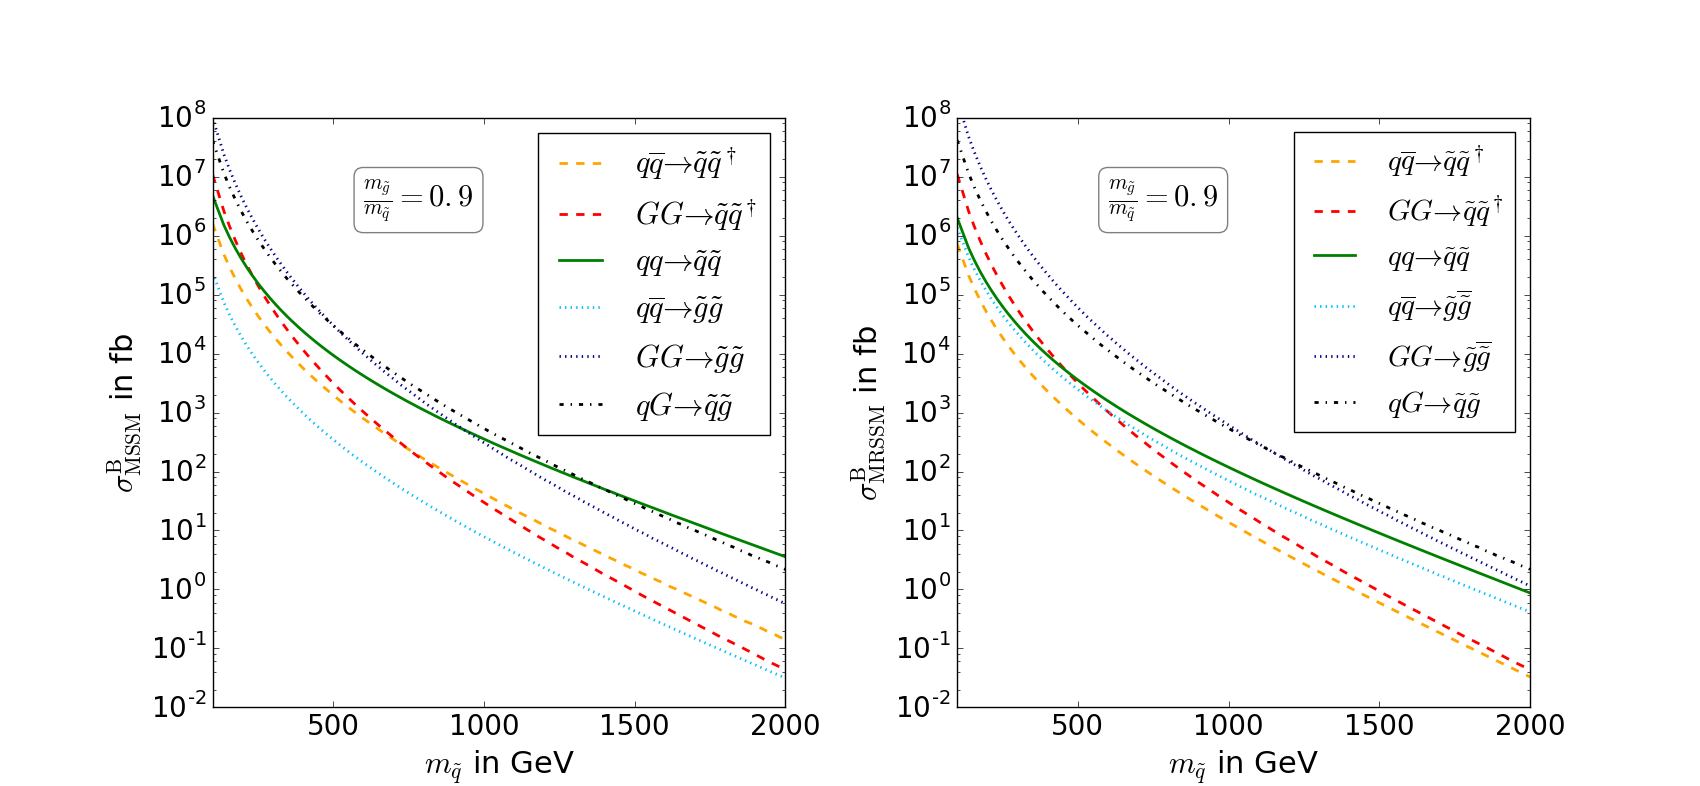
\includegraphics[scale=.45]{figures/mr=0,9_MSSM+MRSSM}
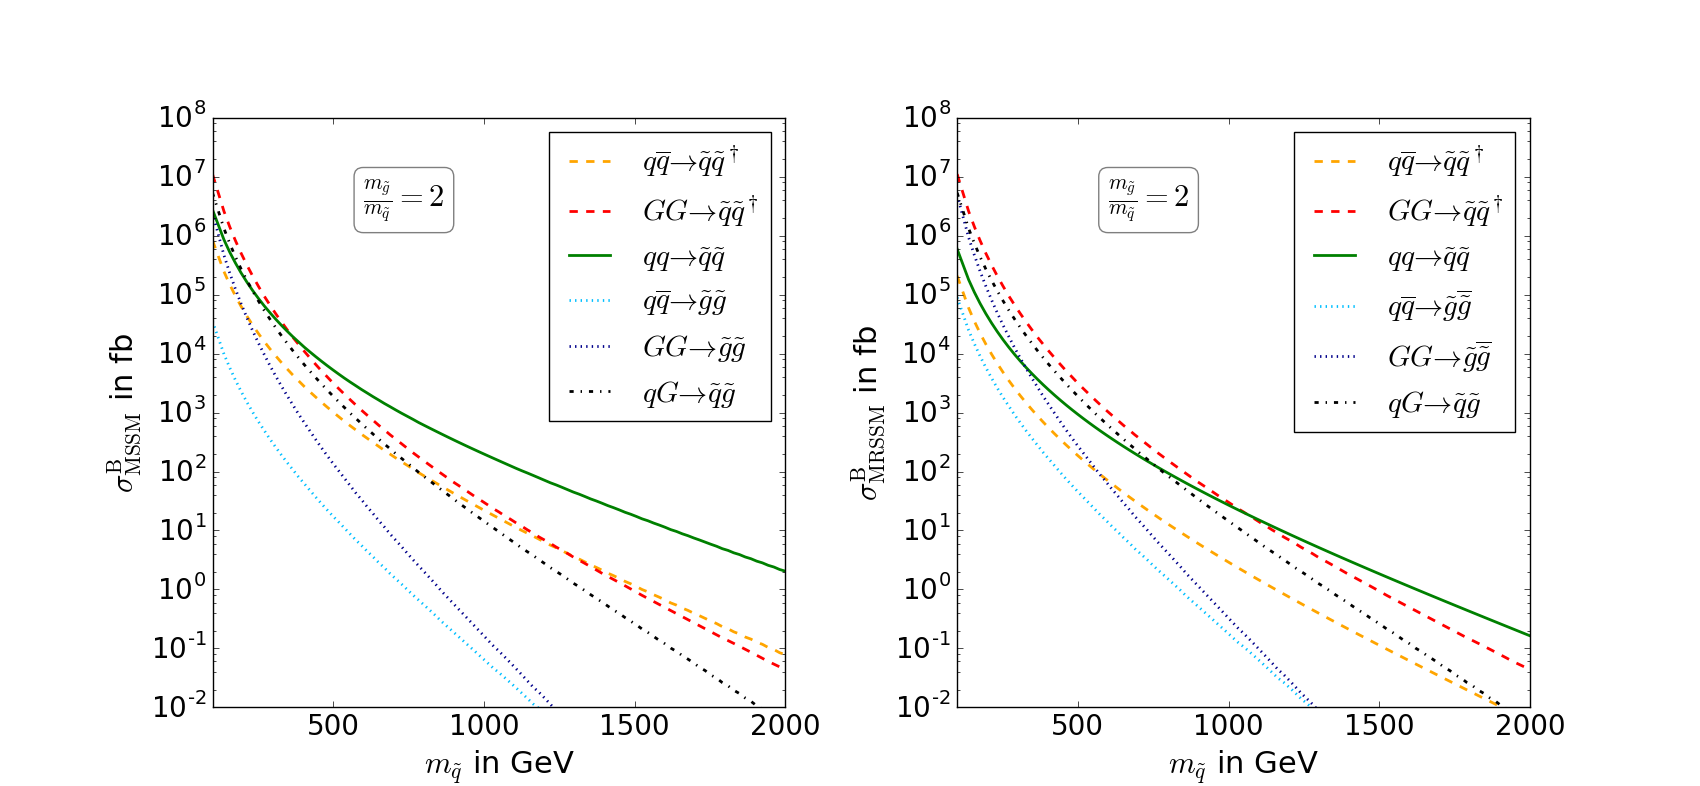
\includegraphics[scale=.45]{figures/mr=2_MSSM+MRSSM}
\end{center}
\end{figure}
\begin{figure}[!htpb]
\begin{center}
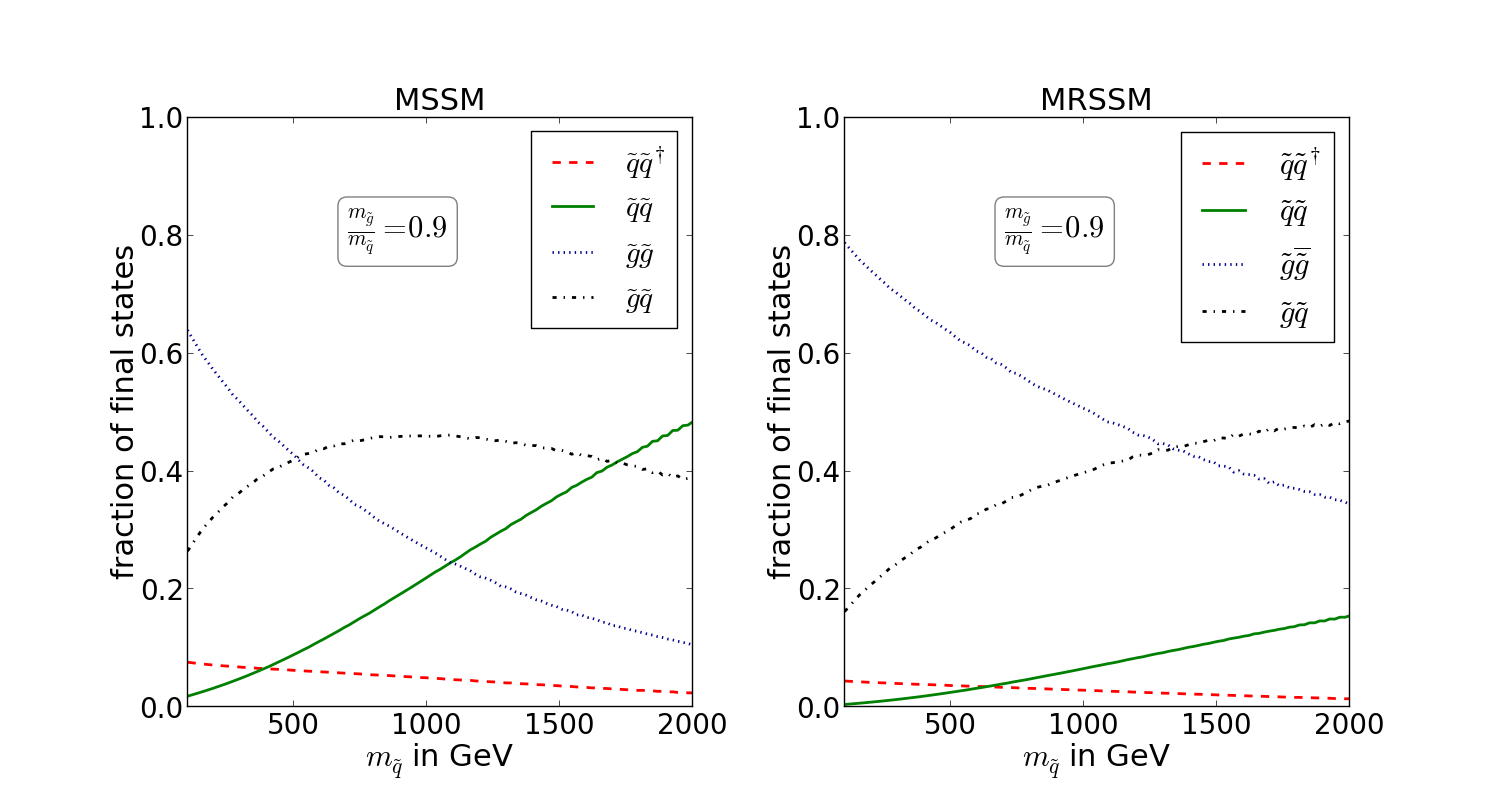
\includegraphics[scale=.45]{figures/rel_weights_mr=0,9_MSSM+MRSSM}
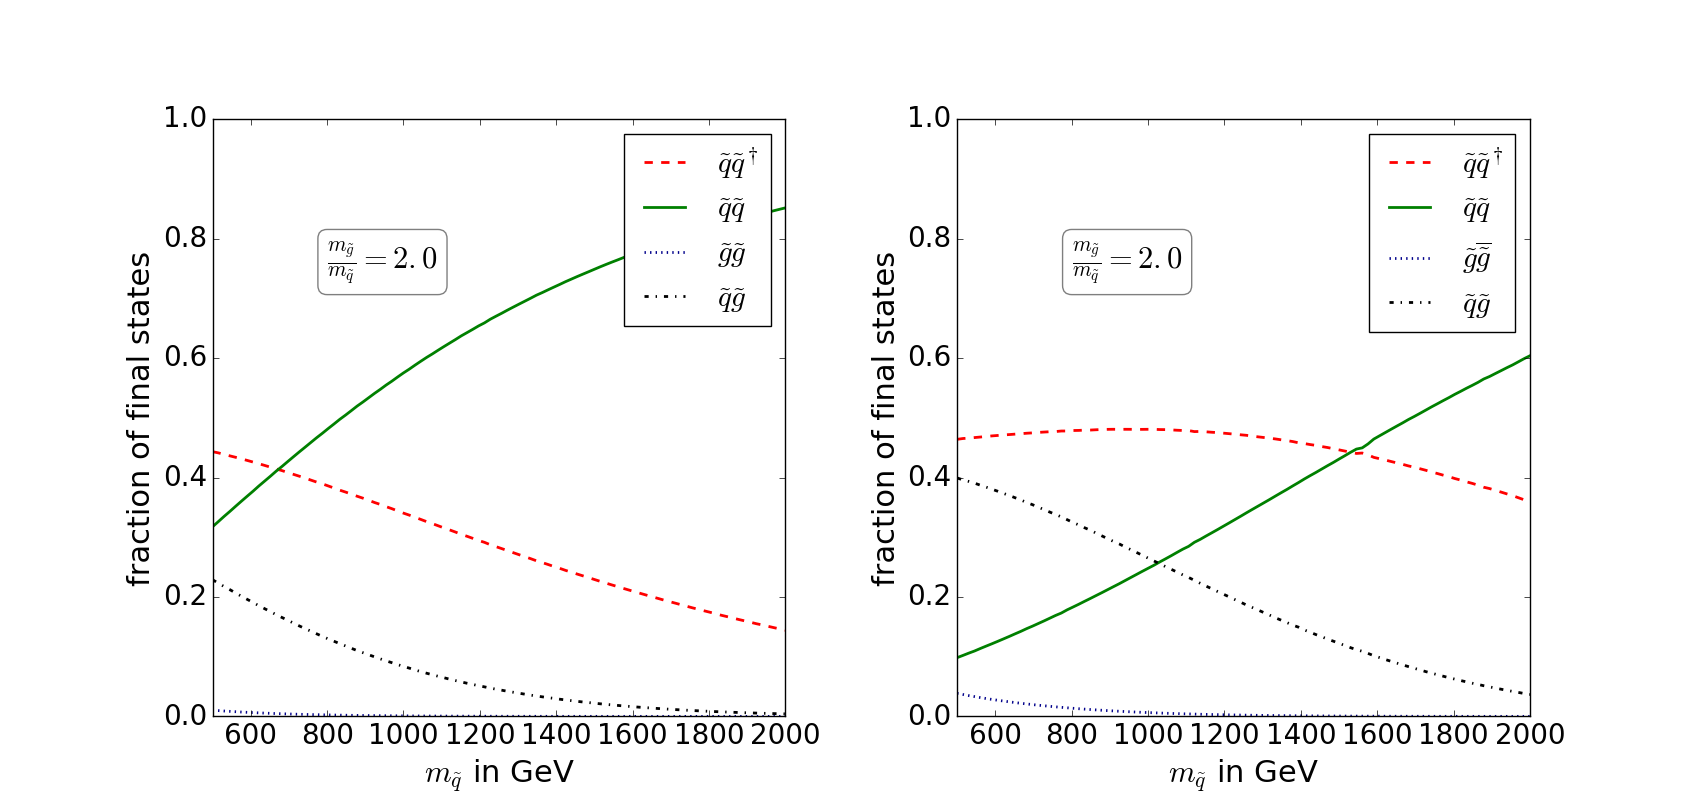
\includegraphics[scale=.45]{figures/rel_weights_mr=2_MSSM+MRSSM}
\end{center}
\end{figure}
\begin{figure}[!htpb]
\begin{center}
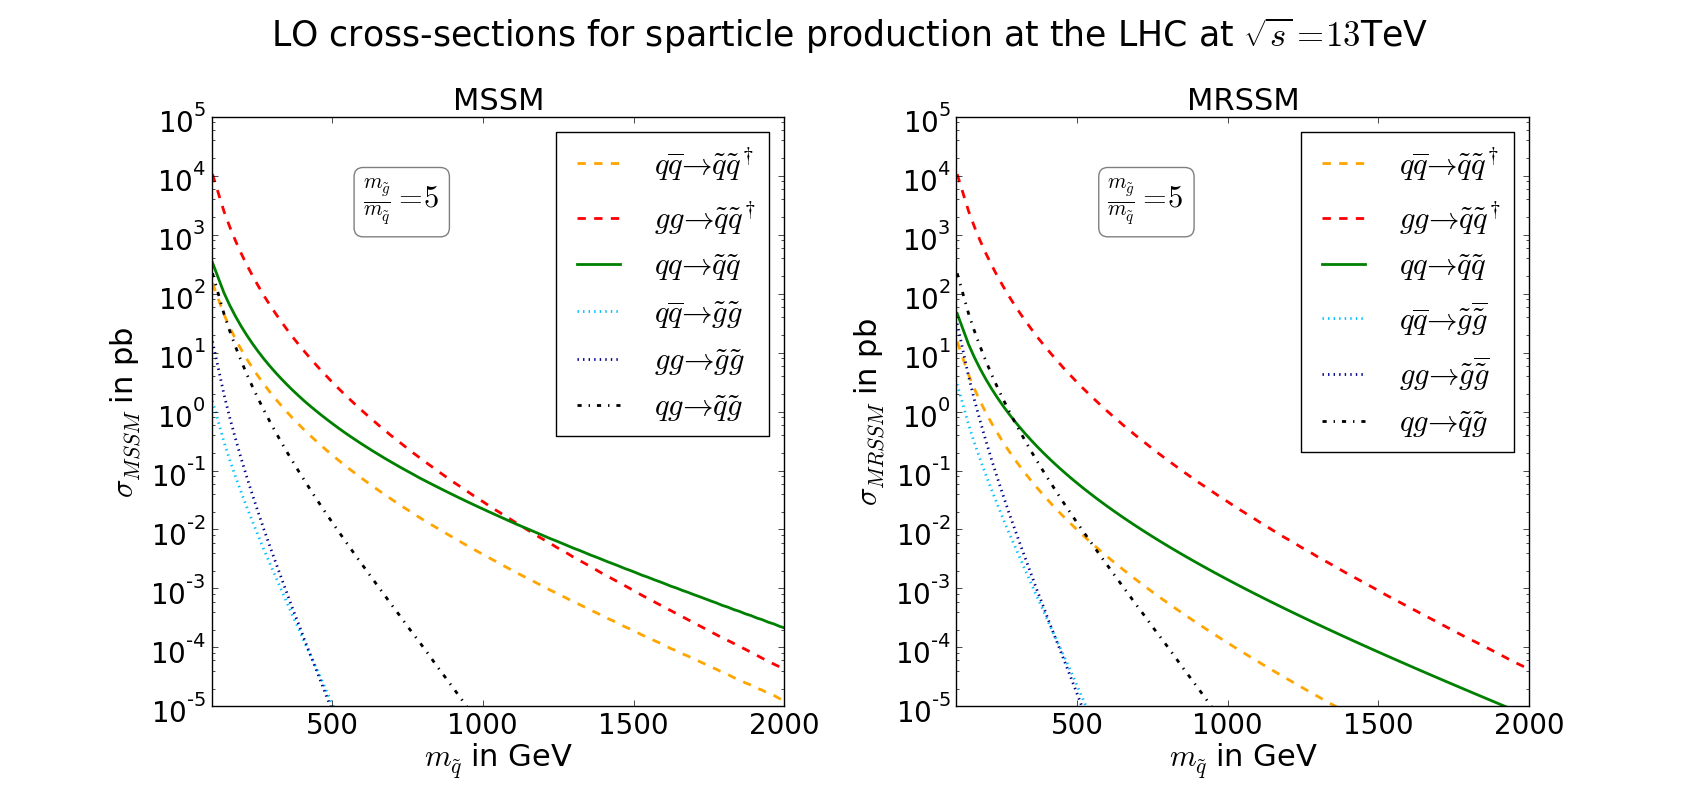
\includegraphics[scale=.45]{figures/mr=5_MSSM+MRSSM}
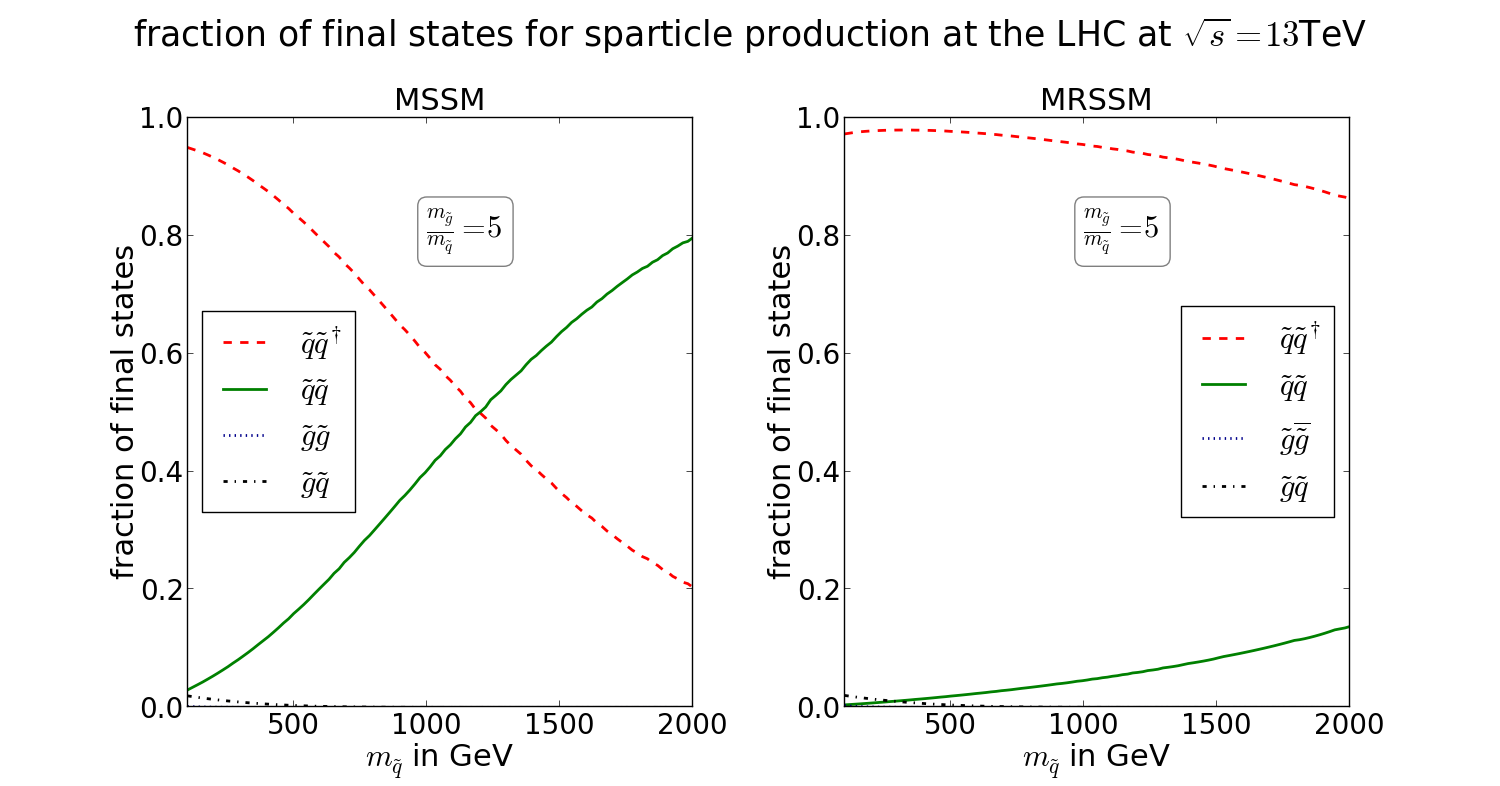
\includegraphics[scale=.45]{figures/rel_weights_mr=5_MSSM+MRSSM}
\end{center}
\end{figure}